%!root = ../main.tex
\chapter{进一步的分析}\label{chap:4.1}
在基础回归的基础上,本文将在基准回归的基础上进行进一步的分析,主要探讨两个问题:第一,灾区家财险保额降低的影响因素可能是什么?第二,居民的行为是否存在一定的异质性?本文将分别从地区异质性、时间异质性、保险标的价值异质性和城乡异质性等方面进行分析。

\section{灾区保额的影响因素:需求的真实下降与保单的理赔不足}

在分析灾区保额在极端天气冲击后降低的现象时,我们可以从两个角度来探讨其可能的影响因素。一个是获得性启发理论\citep{0Do},从居民的心理预期角度来看,当灾区居民经历极端天气事件后,他们可能会重新评估灾害风险,发现实际的损失并没有达到预期的严重程度。这种认知上的变化可能导致他们认为高额的保险投保并不必要,因此选择降低保险额度,以减少未来的保险费用支出。这种心理预期的调整可能是由于居民对灾害的直观感受和对保险赔付能力的初步判断所驱动的。另一个视角是保险公司的逆向选择,从保险市场的运作机制来看,灾区居民可能通过观察和经验发现,保险公司在灾害发生后的赔付比较有限,这可能是由于保险公司巨灾后的赔付策略、资金流动性或风险控制等多种因素造成的\citep{田玲2009中国财产保险业巨灾损失赔付能力实证研究}。当居民意识到即使购买了保险,实际获得的赔付也可能远远低于预期,他们可能会认为保险的经济性不高,从而减少投保额度,以避免支付高额的保险费用而获得较低的保障。

为了深入理解这两种因素对灾区赔付的影响,本文采用DID进行Logit回归分析。回归的因变量之一是“是否理赔”($\text{Claims}$),即保单在灾害发生后是否获得了保险公司的赔付;另一个因变量是“是否续约”($\text{Renew}$),即保单持有者是否选择在第二年继续购买同一保险产品。通过比较灾害发生前后的保险行为变化,我们可以更准确地捕捉到灾害对保险市场的影响。

根据DID Logit回归的结果表\ref{tab:claims},续约的交互项系数为正,这表明在经历了极端天气事件后,灾区居民实际上更愿意续保,这可能是因为他们认识到了灾害风险的严重性。然而,与此同时,保险公司的赔付能力可能并未达到居民的期望,也即巨灾风险暴露与巨灾保险赔付存在不对称\citep{张旭升2010中国巨灾风险暴露与巨灾保险赔付不对称实证},导致他们在续保时选择降低投保额,以减少不必要的保险费用。这也解释了为什么在受灾前的续约系数显著为负,即在没有灾害发生的情况下,居民可能主要因为对保险赔付量的怀疑而不愿意续保。

\begin{table}[H]
    \centering
    \caption{灾区与非灾区赔付/续约DID回归结果}\label{tab:claims}
    
\begin{tabular}{@{\extracolsep{5pt}}lcccc}
\\[-1.8ex]\hline
\hline \\[-1.8ex]
\\[-1.8ex] & \multicolumn{1}{c}{Claim} & \multicolumn{1}{c}{Claim} & \multicolumn{1}{c}{Renew} & \multicolumn{1}{c}{Renew}  \\
\\[-1.8ex] & (1) & (2) & (3) & (4) \\
\hline \\[-1.8ex]
 Disaster & 0.405$^{**}$ & 0.391$^{**}$ & -3.773$^{***}$ & -3.706$^{***}$ \\
& (0.169) & (0.169) & (0.221) & (0.222) \\
 Disaster:Post & 0.630$^{***}$ & 0.622$^{***}$ & 2.243$^{***}$ & 2.232$^{***}$ \\
& (0.190) & (0.190) & (0.234) & (0.235) \\
 Intercept & -6.825$^{***}$ & -4.664$^{***}$ & -5.228$^{***}$ & -11.891$^{***}$ \\
& (0.166) & (0.675) & (0.053) & (0.169) \\
 Post & -0.167$^{}$ & -0.158$^{}$ & -0.556$^{***}$ & -0.525$^{***}$ \\
& (0.123) & (0.123) & (0.028) & (0.029) \\
 Prem\_before & -2.299$^{***}$ & -2.246$^{***}$ & 4.428$^{***}$ & 4.338$^{***}$ \\
& (0.708) & (0.709) & (0.020) & (0.020) \\
 log(Coverage) & & -0.212$^{***}$ & & 0.668$^{***}$ \\
& & (0.067) & & (0.015) \\
 log(GDP) & -0.001$^{}$ & -0.001$^{}$ & 0.013$^{***}$ & 0.013$^{***}$ \\
& (0.006) & (0.006) & (0.002) & (0.002) \\
 log(Penetration) & -0.645$^{***}$ & -0.551$^{***}$ & 2.541$^{***}$ & 2.448$^{***}$ \\
& (0.152) & (0.156) & (0.056) & (0.056) \\
 log(Price) & 0.013$^{}$ & 0.140$^{**}$ & 0.499$^{***}$ & 0.031$^{***}$ \\
& (0.030) & (0.061) & (0.011) & (0.010) \\
\hline \\[-1.8ex]
 Observations & 709271 & 709271 & 709271 & 709271 \\
 Pseudo $R^2$ & 0.012 & 0.013 & 0.368 & 0.377 \\
 Yera FE & True & True & True & True \\
\hline
\hline \\[-1.8ex]
\textit{Note:} & \multicolumn{4}{r}{$^{*}$p$<$0.1; $^{**}$p$<$0.05; $^{***}$p$<$0.01} \\
\end{tabular}

\end{table}

\section{地区异质性:适应性预期造成灾区结果差异}
在探讨极端天气事件对不同地区影响的差异性时,本文首先关注了地区对此类事件的反应是否存在显著的地域性差异。基于东部沿海地区频繁遭受降水事件的影响,居民可能因多次面对风险而逐渐形成了对此类风险的适应性预期。正如台风路径上的企业对自然灾害的反应效率提升\citep{0Do},频繁的降水可能为他们累积了经验,降低了对极端天气的敏感度\citep{陈思柳2021不同决策情境下的损失厌恶效应差异}。
相反,在干旱少雨的西部地区,由于降水事件较为罕见,由于降水相对较少对极端降水风险的敏感度不足,这可能导致他们在面对极端天气时的反应与东部地区存在显著差异。

为了验证这一假设,本研究根据国家统计局的划分标准,将样本划分为东部、中部和西部三个地区,并分别进行了回归分析。回归结果如表\ref{tab:het_geo}所示,基本与表\ref{tab:did1}和表\ref{tab:did2}一致。东部和中部地区在遭受极端降水事件后,灾区交互项系数为负,表明保险金额有所下降,而在近灾区,保险金额的增长更为显著。

\begin{sidewaystable}[htbp]
    \centering
    \caption{分地区回归结果}\label{tab:het_geo}
    
\begin{tabular}{@{\extracolsep{5pt}}lcccccc}
\\[-1.8ex]\hline
\hline \\[-1.8ex]
& \multicolumn{6}{c}{\textit{Dependent variable: log(Coverage)}} \
\cr \cline{2-7}
\\[-1.8ex] & \multicolumn{1}{c}{East} & \multicolumn{1}{c}{Middle} & \multicolumn{1}{c}{West} & \multicolumn{1}{c}{East} & \multicolumn{1}{c}{Middle} & \multicolumn{1}{c}{West}  \\
\\[-1.8ex] & (1) & (2) & (3) & (4) & (5) & (6) \\
\hline \\[-1.8ex]
 Disaster & -0.090$^{***}$ & 0.054$^{***}$ & -0.159$^{***}$ & & & \\
& (0.006) & (0.008) & (0.006) & & & \\
 Disaster:Post & -0.121$^{***}$ & -0.136$^{***}$ & 0.123$^{***}$ & & & \\
& (0.007) & (0.009) & (0.008) & & & \\
 Neighbor & & & & -0.233$^{***}$ & -0.136$^{***}$ & -0.490$^{***}$ \\
& & & & (0.016) & (0.018) & (0.129) \\
 Neighbor:Post & & & & 0.246$^{***}$ & 0.052$^{***}$ & 0.570$^{***}$ \\
& & & & (0.017) & (0.019) & (0.129) \\
 Post & 0.065$^{***}$ & 0.036$^{***}$ & -0.171$^{***}$ & 0.065$^{***}$ & 0.037$^{***}$ & -0.172$^{***}$ \\
& (0.004) & (0.004) & (0.004) & (0.004) & (0.004) & (0.004) \\
%  Prem\_before & 0.185$^{***}$ & 0.107$^{***}$ & 0.067$^{***}$ & 0.174$^{***}$ & 0.106$^{***}$ & 0.071$^{***}$ \\
% & (0.006) & (0.030) & (0.016) & (0.006) & (0.034) & (0.016) \\
%  log(GDP) & 0.000$^{}$ & 0.000$^{}$ & -0.000$^{}$ & 0.000$^{}$ & 0.000$^{}$ & -0.000$^{}$ \\
% & (0.000) & (0.000) & (0.000) & (0.000) & (0.000) & (0.000) \\
%  log(Penetration) & 0.906$^{***}$ & 0.029$^{***}$ & 0.071$^{***}$ & 0.909$^{***}$ & 0.027$^{***}$ & 0.116$^{***}$ \\
% & (0.005) & (0.007) & (0.005) & (0.005) & (0.008) & (0.005) \\
%  log(Price) & 0.312$^{***}$ & 0.684$^{***}$ & 0.848$^{***}$ & 0.296$^{***}$ & 0.672$^{***}$ & 0.852$^{***}$ \\
% & (0.001) & (0.002) & (0.001) & (0.001) & (0.002) & (0.002) \\
Intercept & 11.386$^{***}$ & 9.757$^{***}$ & 9.331$^{***}$ & 11.444$^{***}$ & 9.793$^{***}$ & 9.298$^{***}$ \\
& (0.005) & (0.006) & (0.007) & (0.006) & (0.007) & (0.007) \\
Controls & True & True & True & True & True & True \\
\hline \\[-1.8ex]
 Observations & 481063 & 123513 & 104695 & 450350 & 107232 & 96922 \\
 $R^2$ & 0.333 & 0.593 & 0.764 & 0.314 & 0.585 & 0.774 \\
 Adjusted $R^2$ & 0.333 & 0.592 & 0.764 & 0.314 & 0.585 & 0.774 \\
 Residual Std. Error & 0.704  & 0.439  & 0.375  & 0.718  & 0.447  & 0.364  \\
 F Statistic & 34345.705$^{***}$  & 25654.772$^{***}$  & 48356.638$^{***}$  & 29449.242$^{***}$  & 21634.683$^{***}$  & 47450.879$^{***}$  \\
    Year FE & True & True & True & True & True & True \\
\hline
\hline \\[-1.8ex]
\textit{Note:} & \multicolumn{6}{r}{$^{*}$p$<$0.1; $^{**}$p$<$0.05; $^{***}$p$<$0.01} \\
\end{tabular}

\end{sidewaystable}

然而,在西部地区,极端降水事件冲击导致近灾区的交互项系数显著为负,而灾区的交互项系数则显著为正,这与东部和中部地区的情况形成了鲜明对比。原因可能有两方面:一方面由于西部地区极端降水事件虽然也是二十年一遇,但绝对值相对较低,如图\ref{fig:rainings}所示,风险造成的损失相对有限,因此对居民行为的影响有限,导致远灾区和近灾区的显著性不高,同时回归的数值也相对较小。
另一方面,西部地区居民对极端降水风险的敏感度较低,很难唤醒保险需求,容易低估了极端天气发生的概率\citep{tversky1973availability},导致保险覆盖不足。因此,在巨灾发生后,他们可能有补充保障的动机,这反映在灾区交互项系数显著为正上。


\begin{figure}[H]
    \centering
    \begin{minipage}{0.48\linewidth}
        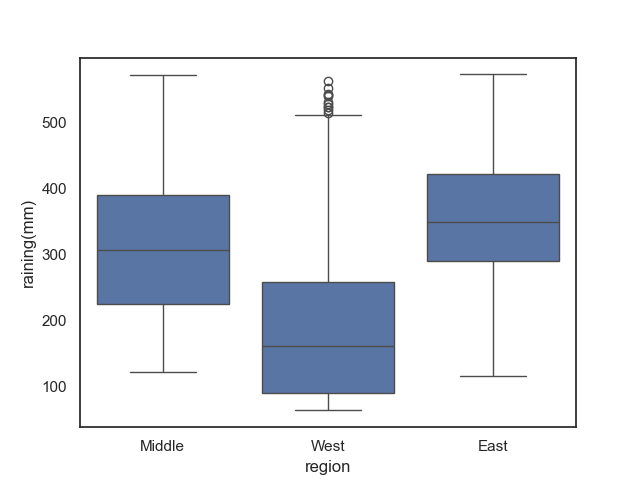
\includegraphics[width=\linewidth]{lib/img/rainings.png}
        \caption{样本中西部地区二十年一遇极端降水事件降水绝对值相对偏低}\label{fig:rainings}
    \end{minipage}
    \begin{minipage}{0.48\linewidth}
        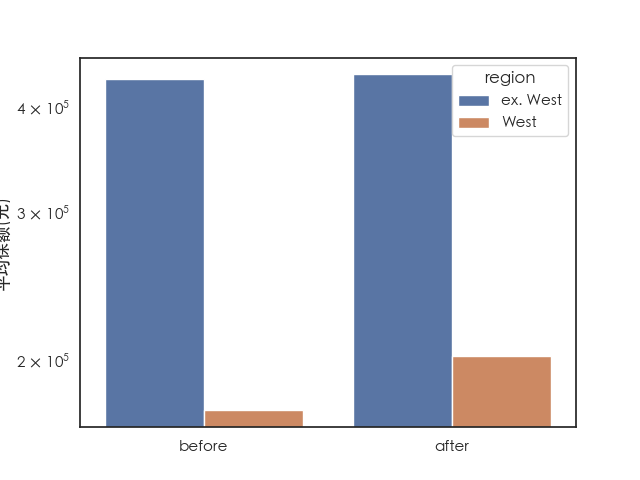
\includegraphics[width=\linewidth]{lib/img/covbyregion.png}
        \caption{西部地区在极端降水发生后有补充保险保障的动机}
    \end{minipage}
\end{figure}

综上所述,本研究的结果揭示了不同地区对极端天气事件的反应确实存在显著的地域性差异。这种差异可能源于地区间对极端天气风险感知程度的不同,进而导致了不同的保险需求水平。但总的来说,这一发现与假设\ref{hyp:3}的预期保持一致,即极端天气事件本质上是通过提高风险感知,导致家财险需求的增加

\section{时间异质性:地震巨灾造成近灾区结果差异}

在探讨极端天气事件对不同时间点的反应差异时,本文以2008年为界,将样本最丰富的时间段分割为2003-2008年和2009-2013年两段,分别代表了两个不同的经济时期,得到的回归结果如表\ref{tab:het_time}所示,也与表\ref{tab:did1}和表\ref{tab:did2}基本一致,即表现为极端天气事件发生后控制组购买家财险的保额普遍提升,但灾区提升相对有限。

\begin{table}[ht]
    \centering
    \renewcommand{\arraystretch}{1}
    \caption{分时间回归结果}\label{tab:het_time}
    
\begin{tabular}{@{\extracolsep{5pt}}lcccc}
\\[-1.8ex]\hline
\hline \\[-1.8ex]
& \multicolumn{4}{c}{\textit{Dependent variable: log(Coverage)}} \
\cr \cline{2-5}
\\[-1.8ex] & \multicolumn{1}{c}{2003-2008} & \multicolumn{1}{c}{2009-2013} & \multicolumn{1}{c}{2003-2008} & \multicolumn{1}{c}{2009-2013}  \\
\\[-1.8ex] & (1) & (2) & (3) & (4) \\
\hline \\[-1.8ex]
 Disaster & 0.017$^{*}$ & -0.013$^{}$ & & \\
& (0.010) & (0.014) & & \\
 Disaster:Post & -0.170$^{***}$ & -0.089$^{***}$ & & \\
& (0.012) & (0.017) & & \\
 Intercept & 11.821$^{***}$ & 12.417$^{***}$ & 11.859$^{***}$ & 12.542$^{***}$ \\
& (0.006) & (0.006) & (0.005) & (0.007) \\
 Neighbor & & & 0.440$^{***}$ & -0.297$^{***}$ \\
& & & (0.012) & (0.043) \\
 Neighbor:Post & & & 0.032$^{*}$ & 0.211$^{***}$ \\
& & & (0.014) & (0.045) \\
 Post & 0.072$^{***}$ & 0.087$^{***}$ & 0.086$^{***}$ & 0.033$^{***}$ \\
& (0.006) & (0.007) & (0.006) & (0.008) \\
%  Prem\_before & 0.196$^{***}$ & 0.784$^{***}$ & 0.336$^{***}$ & 0.768$^{***}$ \\
% & (0.011) & (0.011) & (0.010) & (0.012) \\
%  Price & 0.187$^{***}$ & 0.113$^{***}$ & 0.166$^{***}$ & 0.125$^{***}$ \\
% & (0.001) & (0.001) & (0.001) & (0.001) \\
\hline \\[-1.8ex]
 Observations & 268828 & 191588 & 301508 & 139476 \\
 $R^2$ & 0.102 & 0.156 & 0.119 & 0.183 \\
 Adjusted $R^2$ & 0.102 & 0.156 & 0.119 & 0.183 \\
 Residual Std. Error & 0.982  & 1.058  & 0.998  & 1.045  \\
 F Statistic & 6122.243$^{***}$  & 7057.294$^{***}$  & 8131.866$^{***}$  & 6243.412$^{***}$  \\
\hline
\hline \\[-1.8ex]
\textit{Note:} & \multicolumn{4}{r}{$^{*}$p$<$0.1; $^{**}$p$<$0.05; $^{***}$p$<$0.01} \\
\end{tabular}

\end{table}

值得注意的是,近灾区交互项在2008年后显示出很强的正向提升,这可能是由于2008年汶川大地震使得居民对家庭所在周边的环境更为关注,对极端天气事件的风险感知提升,从而增加了对家财险的需求。并且2008年发生的金融危机也使得家庭对于风险感知更为明显,这一发现也与假设\ref{hyp:3}的预期一致,即极端天气事件通过提高风险感知从而增加家财险需求。

\section{其他异质性分析}
\subsection{保险标的价值异质性}
% 39500.0, 140000.0, 298196.4000000003, 1680000.0
保险标的价值可能对人们的保险购买行为有影响,价值越高的家庭财产在风险意识提升后,保险需求增加的幅度可能更大。本文采用保额的大小作为保险标的价值的代理变量,将样本平均分为低、中、高三组,进行回归分析。其中低保额组的保额在39,500-140,000元,中保额组的保额在140,000-298,196元之间,高保额组的保额在298,196-1,680,000元。回归结果如表\ref{tab:het_cov}所示,近灾区的交互项显示出随保额递增的趋势,说明保额越高,近灾区的保险需求增加越明显,这可能是由于家庭对高价值的家庭财产的损失可能更为敏感,因此保险需求增加的幅度更大。
而对于灾区的交互项系数显示出随保额递减的趋势,也反应灾区灾经历极端天气事件后,由于心理预期及赔付能力的不足,保险需求减少的幅度更大。
\begin{sidewaystable}[ht]
    \centering
    \caption{按保额大小异质性分析}\label{tab:het_cov}
    
\begin{tabular}{@{\extracolsep{5pt}}lcccccc}
\\[-1.8ex]\hline
\hline \\[-1.8ex]
& \multicolumn{6}{c}{\textit{Dependent variable: log(Coverage)}} \
\cr \cline{2-7}
\\[-1.8ex] & \multicolumn{1}{c}{low} & \multicolumn{1}{c}{mid} & \multicolumn{1}{c}{high} & \multicolumn{1}{c}{low} & \multicolumn{1}{c}{mid} & \multicolumn{1}{c}{high}  \\
\\[-1.8ex] & (1) & (2) & (3) & (4) & (5) & (6) \\
\hline \\[-1.8ex]
 Disaster & -0.013$^{***}$ & 0.017$^{***}$ & -0.066$^{***}$ & & & \\
& (0.003) & (0.002) & (0.004) & & & \\
 Disaster:Post & -0.003$^{}$ & -0.033$^{***}$ & -0.117$^{***}$ & & & \\
& (0.004) & (0.003) & (0.005) & & & \\
 Neighbor & & & & 0.096$^{***}$ & -0.060$^{***}$ & -0.115$^{***}$ \\
& & & & (0.007) & (0.006) & (0.023) \\
 Neighbor:Post & & & & -0.099$^{***}$ & 0.064$^{***}$ & 0.138$^{***}$ \\
& & & & (0.008) & (0.006) & (0.024) \\
 Post & 0.017$^{***}$ & 0.017$^{***}$ & 0.009$^{***}$ & 0.018$^{***}$ & 0.017$^{***}$ & 0.008$^{***}$ \\
& (0.002) & (0.002) & (0.003) & (0.002) & (0.002) & (0.003) \\
%  Prem\_before & 0.117$^{***}$ & 0.028$^{***}$ & 0.015$^{***}$ & 0.114$^{***}$ & 0.029$^{***}$ & 0.008$^{**}$ \\
% & (0.005) & (0.003) & (0.004) & (0.005) & (0.002) & (0.004) \\
%  log(GDP) & 0.000$^{**}$ & -0.000$^{}$ & 0.000$^{}$ & 0.000$^{**}$ & -0.000$^{}$ & 0.000$^{*}$ \\
% & (0.000) & (0.000) & (0.000) & (0.000) & (0.000) & (0.000) \\
%  log(Penetration) & 0.123$^{***}$ & 0.083$^{***}$ & 0.158$^{***}$ & 0.126$^{***}$ & 0.077$^{***}$ & 0.146$^{***}$ \\
% & (0.003) & (0.002) & (0.003) & (0.003) & (0.002) & (0.004) \\
%  log(Price) & 0.086$^{***}$ & 0.028$^{***}$ & 0.071$^{***}$ & 0.080$^{***}$ & 0.025$^{***}$ & 0.067$^{***}$ \\
% & (0.001) & (0.000) & (0.001) & (0.001) & (0.000) & (0.001) \\
Intercept & 11.207$^{***}$ & 12.063$^{***}$ & 12.668$^{***}$ & 11.226$^{***}$ & 12.071$^{***}$ & 12.685$^{***}$ \\
& (0.003) & (0.002) & (0.004) & (0.003) & (0.002) & (0.004) \\
Controls & True & True & True & True & True & True \\
\hline \\[-1.8ex]
 Observations & 232914 & 217205 & 214095 & 211102 & 199829 & 200904 \\
 $R^2$ & 0.072 & 0.033 & 0.081 & 0.068 & 0.030 & 0.074 \\
 Adjusted $R^2$ & 0.072 & 0.033 & 0.081 & 0.068 & 0.030 & 0.074 \\
 Residual Std. Error & 0.284  & 0.182  & 0.311  & 0.284  & 0.183  & 0.316  \\
 F Statistic & 2570.208$^{***}$  & 1053.810$^{***}$  & 2706.248$^{***}$  & 2205.864$^{***}$  & 893.130$^{***}$  & 2291.168$^{***}$  \\
 Year FE & True & True & True & True & True & True \\
\hline
\hline \\[-1.8ex]
\textit{Note:} & \multicolumn{6}{r}{$^{*}$p$<$0.1; $^{**}$p$<$0.05; $^{***}$p$<$0.01} \\
\end{tabular}

\end{sidewaystable}

\subsection{城乡异质性}
我国仍面临一定程度的城乡二元化的问题,城市居民和农村居民在收入、教育、医疗、社会保障等方面存在较大差异,这可能导致他们对极端天气事件的风险感知程度不同,进而影响他们的保险需求。本文将样本分为城市(包含各地级市区)和农村(含县区)两组,进行回归分析。回归结果如表\ref{tab:het_rur}所示。城市居民与此前DID回归(见表\ref{tab:did1}及表\ref{tab:did2})基本一致,但是农村灾区和近灾区的交互项绝对值相比于城市更低。这可能一方面由于农村居民与农业关系更密切,对极端天气事件的风险感知程度更高,并且农村基础设施较差、受二十年一遇降水的冲击可能更严重。另一方面由于农村居民的家庭财产保险覆盖率相对较低,且通过农险覆盖了房屋之外的部分风险\citep{falco2014crop,胡新艳2021气候变化,TJLT202108007},因此对家财险的接受程度更低,农村家财险投保样本仅占总样本的约1/3。

\begin{table}[ht]
    \centering
    \caption{按城乡异质性分析}\label{tab:het_rur}
    
\begin{tabular}{@{\extracolsep{5pt}}lcccc}
\\[-1.8ex]\hline
\hline \\[-1.8ex]
& \multicolumn{4}{c}{\textit{Dependent variable: log(Coverage)}} \
\cr \cline{2-5}
\\[-1.8ex] & \multicolumn{1}{c}{农村} & \multicolumn{1}{c}{农村} & \multicolumn{1}{c}{城市} & \multicolumn{1}{c}{城市}  \\
\\[-1.8ex] & (1) & (2) & (3) & (4) \\
\hline \\[-1.8ex]
 Disaster & -0.022$^{*}$ & & 0.283$^{***}$ & \\
& (0.013) & & (0.011) & \\
 Disaster:Post & 0.115$^{***}$ & & -0.543$^{***}$ & \\
& (0.016) & & (0.014) & \\
 Intercept & 12.094$^{***}$ & 12.094$^{***}$ & 12.206$^{***}$ & 12.206$^{***}$ \\
& (0.007) & (0.007) & (0.006) & (0.006) \\
 Neighbor & & -0.120$^{***}$ & & 0.358$^{***}$ \\
& & (0.021) & & (0.016) \\
 Neighbor:Post & & 0.143$^{***}$ & & 0.106$^{***}$ \\
& & (0.024) & & (0.018) \\
 Post & -0.022$^{***}$ & -0.022$^{***}$ & 0.140$^{***}$ & 0.140$^{***}$ \\
& (0.008) & (0.007) & (0.007) & (0.007) \\
\hline \\[-1.8ex]
 Observations & 160810 & 148210 & 317651 & 304242 \\
 $R^2$ & 0.001 & 0.000 & 0.005 & 0.013 \\
 Adjusted $R^2$ & 0.001 & 0.000 & 0.005 & 0.013 \\
 Residual Std. Error & 1.027  & 1.017  & 1.216  & 1.195  \\
 F Statistic & 40.420$^{***}$  & 12.639$^{***}$  & 554.450$^{***}$  & 1304.637$^{***}$  \\
\hline
\hline \\[-1.8ex]
\textit{Note:} & \multicolumn{4}{r}{$^{*}$p$<$0.1; $^{**}$p$<$0.05; $^{***}$p$<$0.01} \\
\end{tabular}

\end{table}
